\documentclass{beamer}
\usetheme{Madrid}

\usepackage{amsmath, amssymb, amsthm}
\usepackage{graphicx}
\usepackage{listings}
\usepackage{gensymb}
\usepackage[utf8]{inputenc}
\usepackage{hyperref}
\usepackage{gvv}

\begin{document}

\title{matgeo: 3.3.4}
\author{EE24BTECH11009 - Mokshith Kumar$^{}$% <-this % stops a space
}
\frame{\titlepage}
\begin{frame}
\frametitle{Question}
Construct a right triangle in which sides (other than the hypotenuse) are $8$cm and $6$cm.\hfill{3.3.4}
\end{frame}
\begin{frame}{allowframebreaks}
\frametitle{Table}
\begin{table}[h]
    \centering
    \begin{tabular}{|c|c|}
        \hline
        Point & Coordinates\\
        \hline
        $A$ & \myvec{0\\6}\\
        \hline
        $B$ & \myvec{8\\0}\\
        \hline
        $C$ & \myvec{0\\0}\\
        \hline
\end{tabular}

    \caption{1}
    \label{table}
\end{table}
\end{frame}
\begin{frame}{allowframebreaks}
\frametitle{Graph}
From \tabref{table},\figref{stemplot} is plotted.
\begin{figure}[h!]
   \centering
   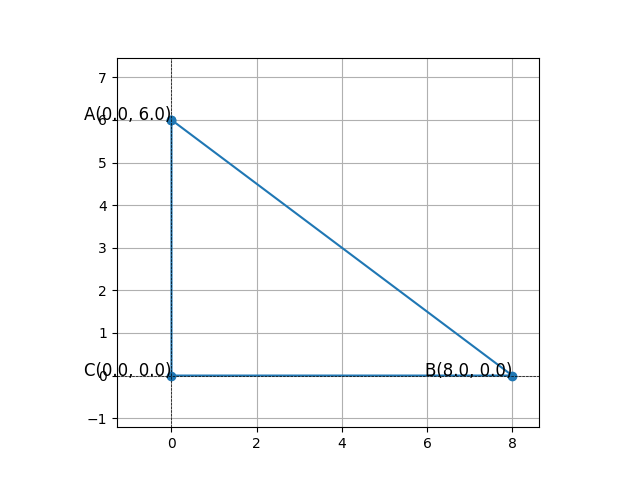
\includegraphics[width=0.7\linewidth]{figs/plot.png}
   \caption{1 }
   \label{stemplot}
\end{figure}\\
\end{frame}
\end{document}